
\chapter{Sprint 3 : Suivi et Création des Rapports}

\section*{Introduction}
\addcontentsline{toc}{section}{Introduction}

Le sprint 3 se concentre sur l'amélioration de la communication et de la visibilité au sein de l'équipe à travers quatre principales fonctionnalités : les notifications, le suivi en temps réel des véhicules, la planification des déplacements et la génération de rapports détaillés pour les interventions. Ce sprint inclut des sections détaillées avec des diagrammes pour clarifier les besoins et processus. La phase de "Réalisation" se concentre sur l'implémentation des fonctionnalités, tandis que la "Rétrospective" et les "Tests unitaires" évaluent les méthodes de développement pour assurer la qualité du produit.

%________________________________________________________________________________________________________________

\section{Backlog du sprint 3}

\begin{table}[htbp]
    \centering
    \renewcommand{\arraystretch}{1.2} % Facteur d'étirement des lignes
    \begin{tabular}{|c|c|p{7.8cm}|p{1cm}|}
        \hline
        \textbf{ID}   & \textbf{Fonctionnalités}       & \centering \textbf{User Story}                                                                                                                          & \textbf { Story points} \\
        \hline

        \textbf{US11} & Suivi en temps réel            & En tant que Chef d'équipe je veux suivre le progrès et la localisation des voiture .                                                                    & 8                       \\
        \hline
        \textbf{US12} & Planification des déplacements & En tant que chauffeur, je veux planifier des voyages pour optimiser mes itinéraires et mes arrêts.                                                      & 5                       \\
        \hline
        \textbf{US13} & Notifications                  & En tant qu’administrateur, chauffeur, mécanicien ou chef d’équipe, je veux recevoir des notifications pour être informé en temps réel des mises à jour. & 5                       \\
        \hline
        \textbf{US14} & Création des rapports          & En tant que Mécanicien je veux Générer des rapports pour que je puisse documenter les détails de chaque intervention .                                  & 3                       \\
        \hline
    \end{tabular}
    \caption{Backlog du sprint 3}

\end{table}
%________________________________________________________________________________________________________________

\section{Analyse et conception}

Nous mettrons en avant le diagramme de cas d'utilisation globale, illustrant les interactions principales des utilisateurs avec le système. Ensuite, pour chaque fonctionnalité identifiée, nous élaborerons des cas d'utilisation spécifiques, accompagnés de diagrammes de séquence système pour détailler l'ordre des opérations. Enfin, nous fournirons une description textuelle détaillée pour chaque cas d'utilisation, décrivant les étapes, les actions et les résultats attendus.
%________________________________________________________________________________________________________________

\subsection{Diagramme de cas d’utilisation du sprint 3}

Ce diagramme de cas d'utilisation présente les interactions des différents acteurs avec le système pour le Sprint 3, qui se concentre sur les fonctionnalités de suivi en temps réel, de consultation des notifications et de création de rapports. \\
Les actions des utilisateurs nécessitent une authentification avant d'accéder à leurs fonctionnalités spécifiques.

\begin{figure}[h!]
    \centering
    \includegraphics[width=1\textwidth,height=14cm]{chap5.images/dcu global sprint 3.png}
    \caption{Diagramme de cas d’utilisation global du sprint 3}

\end{figure}

%________________________________________________________________________________________________________________

\newpage
\subsection{Description textuelle du cas d’utilisation « Suivi en Temps Réel par Géolocalisation »}


\begin{table}[H]
    \centering
    \renewcommand{\arraystretch}{0.9}
    \begin{tabular}{|p{4cm}|p{9cm}|}
        \hline
        \textbf{Cas d'utilisation} & Suivre en temps réel                                                                                           \\
        \hline
        \textbf{Acteur}            & Chef d'équipe et Chauffeur                                                                                     \\
        \hline
        \textbf{Pré-condition}     & 1- Le chauffeur doit être authentifié dans l'application mobile.\newline

        2- Le chauffeur doit avoir activé le suivi GPS sur son téléphone.\newline

        3-Le chef d'équipe doit être authentifié dans l'application mobile et avoir accès à l'interface de suivi en temps réel.                     \\


        \hline
        \textbf{Post-condition}    & 1- Le chef peut suivre la position du camion en temps réel sur la carte.
        \newline

        2- Le chauffeur peut pinner les lieux où il fait une pause ou où il remplit du carburant.\newline

        3- Les pins apparaissent en temps réel sur la carte du chef.                                                                                \\
        \hline
        \textbf{Scénario nominal}  & 1- Le chauffeur s'authentifie dans l'application mobile (appel au cas d'utilisation "S'authentifier").\newline

        2- Le chauffeur active le suivi GPS.\newline

        3- Le chauffeur planifie les déplacements avant son départ (appel au cas d’utilisation "Planifier les déplacements").\newline

        4- Le chef s'authentifie dans l'application (appel au cas d'utilisation "S'authentifier").\newline

        5- Le chef accède à l'interface de suivi en temps réel.\newline

        6- Le système vérifie la position actuelle du camion et l'affiche sur la carte.\newline
        \\
    \end{tabular}

\end{table}





\begin{table}[H]
    \centering
    \renewcommand{\arraystretch}{1}
    \begin{tabular}{|p{4cm}|p{9cm}|}



                                     & 7- Le chef voit l'emplacement marqué en temps réel sur la carte. \\


        \hline
        \textbf{Scénario alternatif} & A1 Position GPS non disponible : \newline

        l'enchainement A1 démarre au point 5 du scénario nominal.\newline

        6- Un message d'erreur s'affiche, indiquant que la position GPS n'est pas disponible.. \newline

        Le scénario nominal reprend au point 2.                                                         \\

        \hline
    \end{tabular}
    \caption{Description textuelle du cas d’utilisation “Suivi en Temps Réel par Géolocalisation”}

\end{table}



%________________________________________________________________________________________________________________

\subsection{Description textuelle du cas d’utilisation « Planifier les déplacements »}

\begin{table}[htbp]
    \centering
    \renewcommand{\arraystretch}{1.5}
    \begin{tabular}{|p{4cm}|p{9.5cm}|}
        \hline
        \textbf{Cas d'utilisation}   & Planifier les déplacements                                                                                 \\
        \hline
        \textbf{Acteur}              & Chauffeur                                                                                                  \\
        \hline
        \textbf{Pré-condition}       & Le chauffeur doit être connecté à l'application  .                                                         \\


        \hline
        \textbf{Post-condition}      & Les détails du trajet choisi, des pauses et des arrêts pour le carburant sont enregistrés dans le système. \\
        \hline
        \textbf{Scénario nominal}    & 1- Le chauffeur sélectionne le trajet optimal sur la carte .\newline

        2- Pendant le trajet, le chauffeur peut localiser les différentes stations de carburant à proximité du trajet prévu.\newline

        3- Le système vérifie le trajet, l'enregistre, et le marque sur la carte.\newline

        4- Toutes les actions sont mises à jour en temps réel sur la carte.
        \\
        \hline
        \textbf{Scénario alternatif} & A1 Erreur de vérification du trajet : \newline

        l'enchainement A1 démarre au point 3 du scénario nominal.\newline

        4- Un message d'erreur s'affiche pour vérifier le trajet sélectionné. \newline

        Le scénario nominal reprend au point 1.                                                                                                   \\
        \hline
    \end{tabular}
    \caption{Description textuelle du cas d’utilisation “ Planifier les déplacements ”}
\end{table}



%________________________________________________________________________________________________________________
\newpage

\subsection{Description textuelle du cas d’utilisation « Consulter Notifications »}

\begin{table}[htbp]
    \centering
    \renewcommand{\arraystretch}{1.5}
    \begin{tabular}{|p{4cm}|p{9.5cm}|}
        \hline
        \textbf{Cas d'utilisation} & Consulter les notifications                                                                              \\
        \hline
        \textbf{Acteur}            & Administrateur, Chef d’équipe, Chauffeur et Mécanicien                                                   \\
        \hline
        \textbf{Pré-condition}     & 1- L'utilisateur doit être authentifié dans l'application mobile.\newline

        2- L'utilisateur doit avoir accès à l'interface de consultation des notifications.                                                    \\


        \hline
        \textbf{Post-condition}    & L'utilisateur peut voir toutes les notifications.                                                        \\
        \hline
        \textbf{Scénario nominal}  & 1- L'utilisateur s'authentifie dans l'application (appel au cas d'utilisation "S'authentifier").\newline

        2- L'utilisateur accède à l'interface de consultation des notifications.\newline

        3- Le système affiche la liste des notifications, triées par ordre chronologique.                                                     \\

        \hline
    \end{tabular}
    \caption{Description textuelle du cas d’utilisation “ Consulter Notifications ”}

\end{table}


\subsection{Diagramme d'activité du cas d’utilisation « Consulter Notifications »}


\begin{figure}[ht!]
    \centering
    \includegraphics[width=0.9\textwidth,height=10cm]{chap5.images/notif activité.png}
    \caption{ Diagramme d'activité du cas d’utilisation « Consulter Notifications » }
\end{figure}




%________________________________________________________________________________________________________________
\newpage
\subsection{Raffinement du cas d'utilisation « Générer des rapports »}

\begin{figure}[h!]
    \centering
    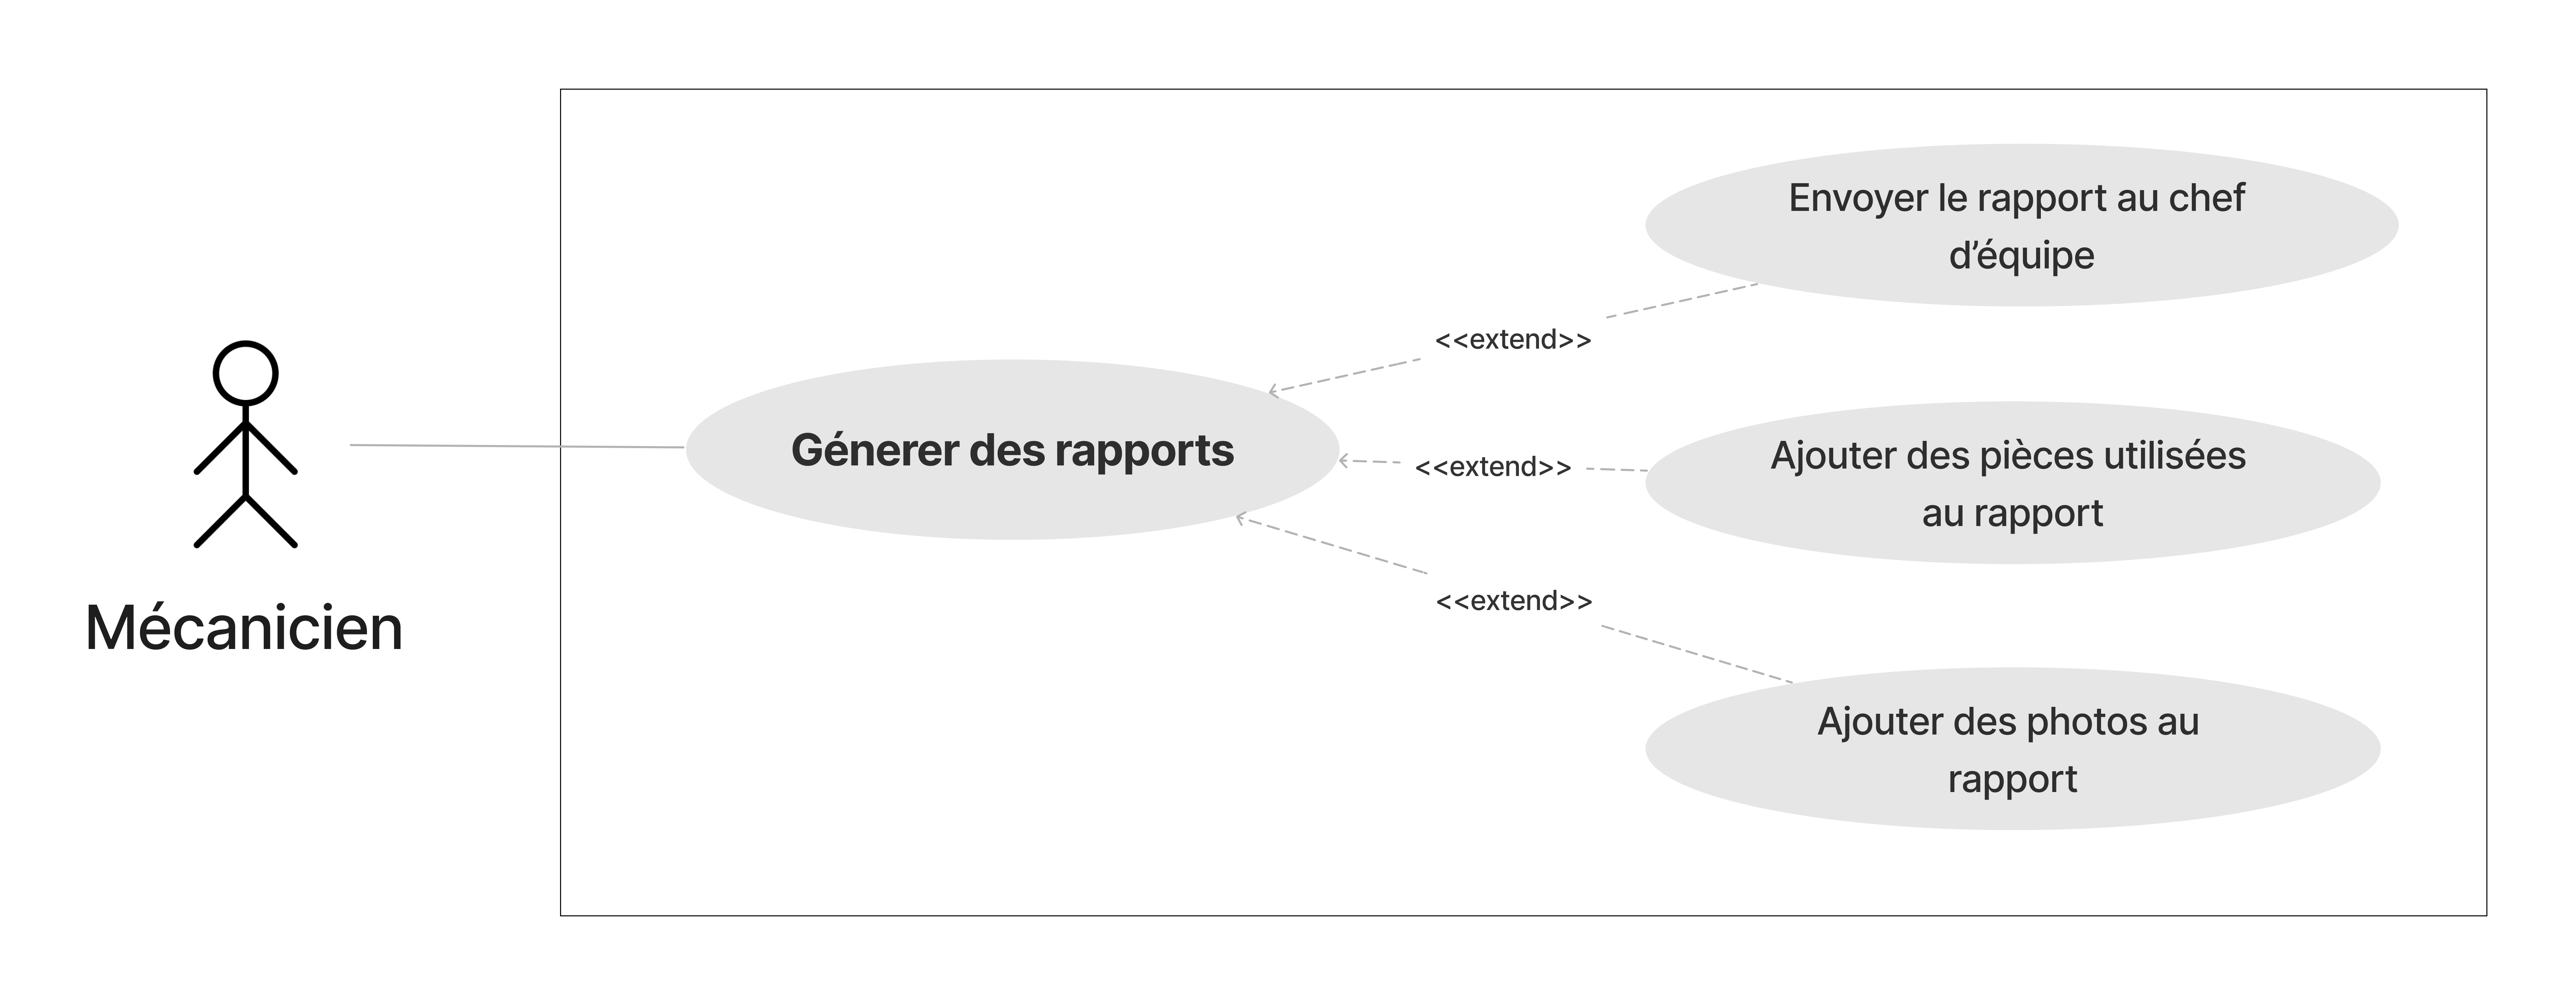
\includegraphics[width=1\textwidth,height=5.5cm]{chap5.images/raff generer rapport.png}
    \caption{ Raffinement du cas d'utilisation « Générer des rapports » }
\end{figure}

\subsection{Description textuelle du cas d’utilisation « Générer des rapports »}

\begin{table}[H]
    \centering
    \renewcommand{\arraystretch}{1}
    \begin{tabular}{|p{4cm}|p{9cm}|}
        \hline
        \textbf{Cas d'utilisation} & Écrire des rapports                                                                                              \\
        \hline
        \textbf{Acteur}            & Mécanicien                                                                                                       \\
        \hline
        \textbf{Pré-condition}     & Le mécanicien doit être authentifié dans l'application mobile et a l'accès à l'interface de saisie des rapports. \\


        \hline
        \textbf{Post-condition}    & 1-Le rapport est enregistré dans le système avec tous les détails requis.\newline

        2- Les rapports existants s'affichent dans l'interface en dessous du formulaire de saisie.                                                    \\
        \hline
        \textbf{Scénario nominal}  & 1- Le mécanicien s'authentifie dans l'application mobile (appel au cas d'utilisation "S'authentifier").\newline

        2- Le mécanicien accède à l'interface de saisie des rapports.\newline

        3- Le mécanicien saisit la matricule du véhicule.\newline

        4- Le mécanicien entre les détails de l'intervention (description des travaux effectués, pièces remplacées).\newline

        5- Le mécanicien appuie sur le bouton "Confirmer le rapport".\newline

        6- Le système vérifie la matricule du véhicule.                                                                                               \\
    \end{tabular}
\end{table}

\newpage

\begin{table}[H]
    \centering
    \renewcommand{\arraystretch}{0.9}
    \begin{tabular}{|p{4cm}|p{9cm}|}



                                     & 7- Le système enregistre les informations saisies et génère un rapport. \\

        \hline
        \textbf{Scénario alternatif} & A1 Erreur de saisie de la matricule :\newline

        l'enchainement A1 démarre au point 6 du scénario nominal.\newline

        4- un message d'erreur va etre afficher. \newline

        Le scénario nominal reprend au point 3.                                                                \\

        \hline
    \end{tabular}
    \caption{Description textuelle du cas d’utilisation “ Générer des rapports ”}

\end{table}

\subsection{Diagramme de séquence système du cas d’utilisation « Générer des rapports »}

\begin{figure}[h!]
    \centering
    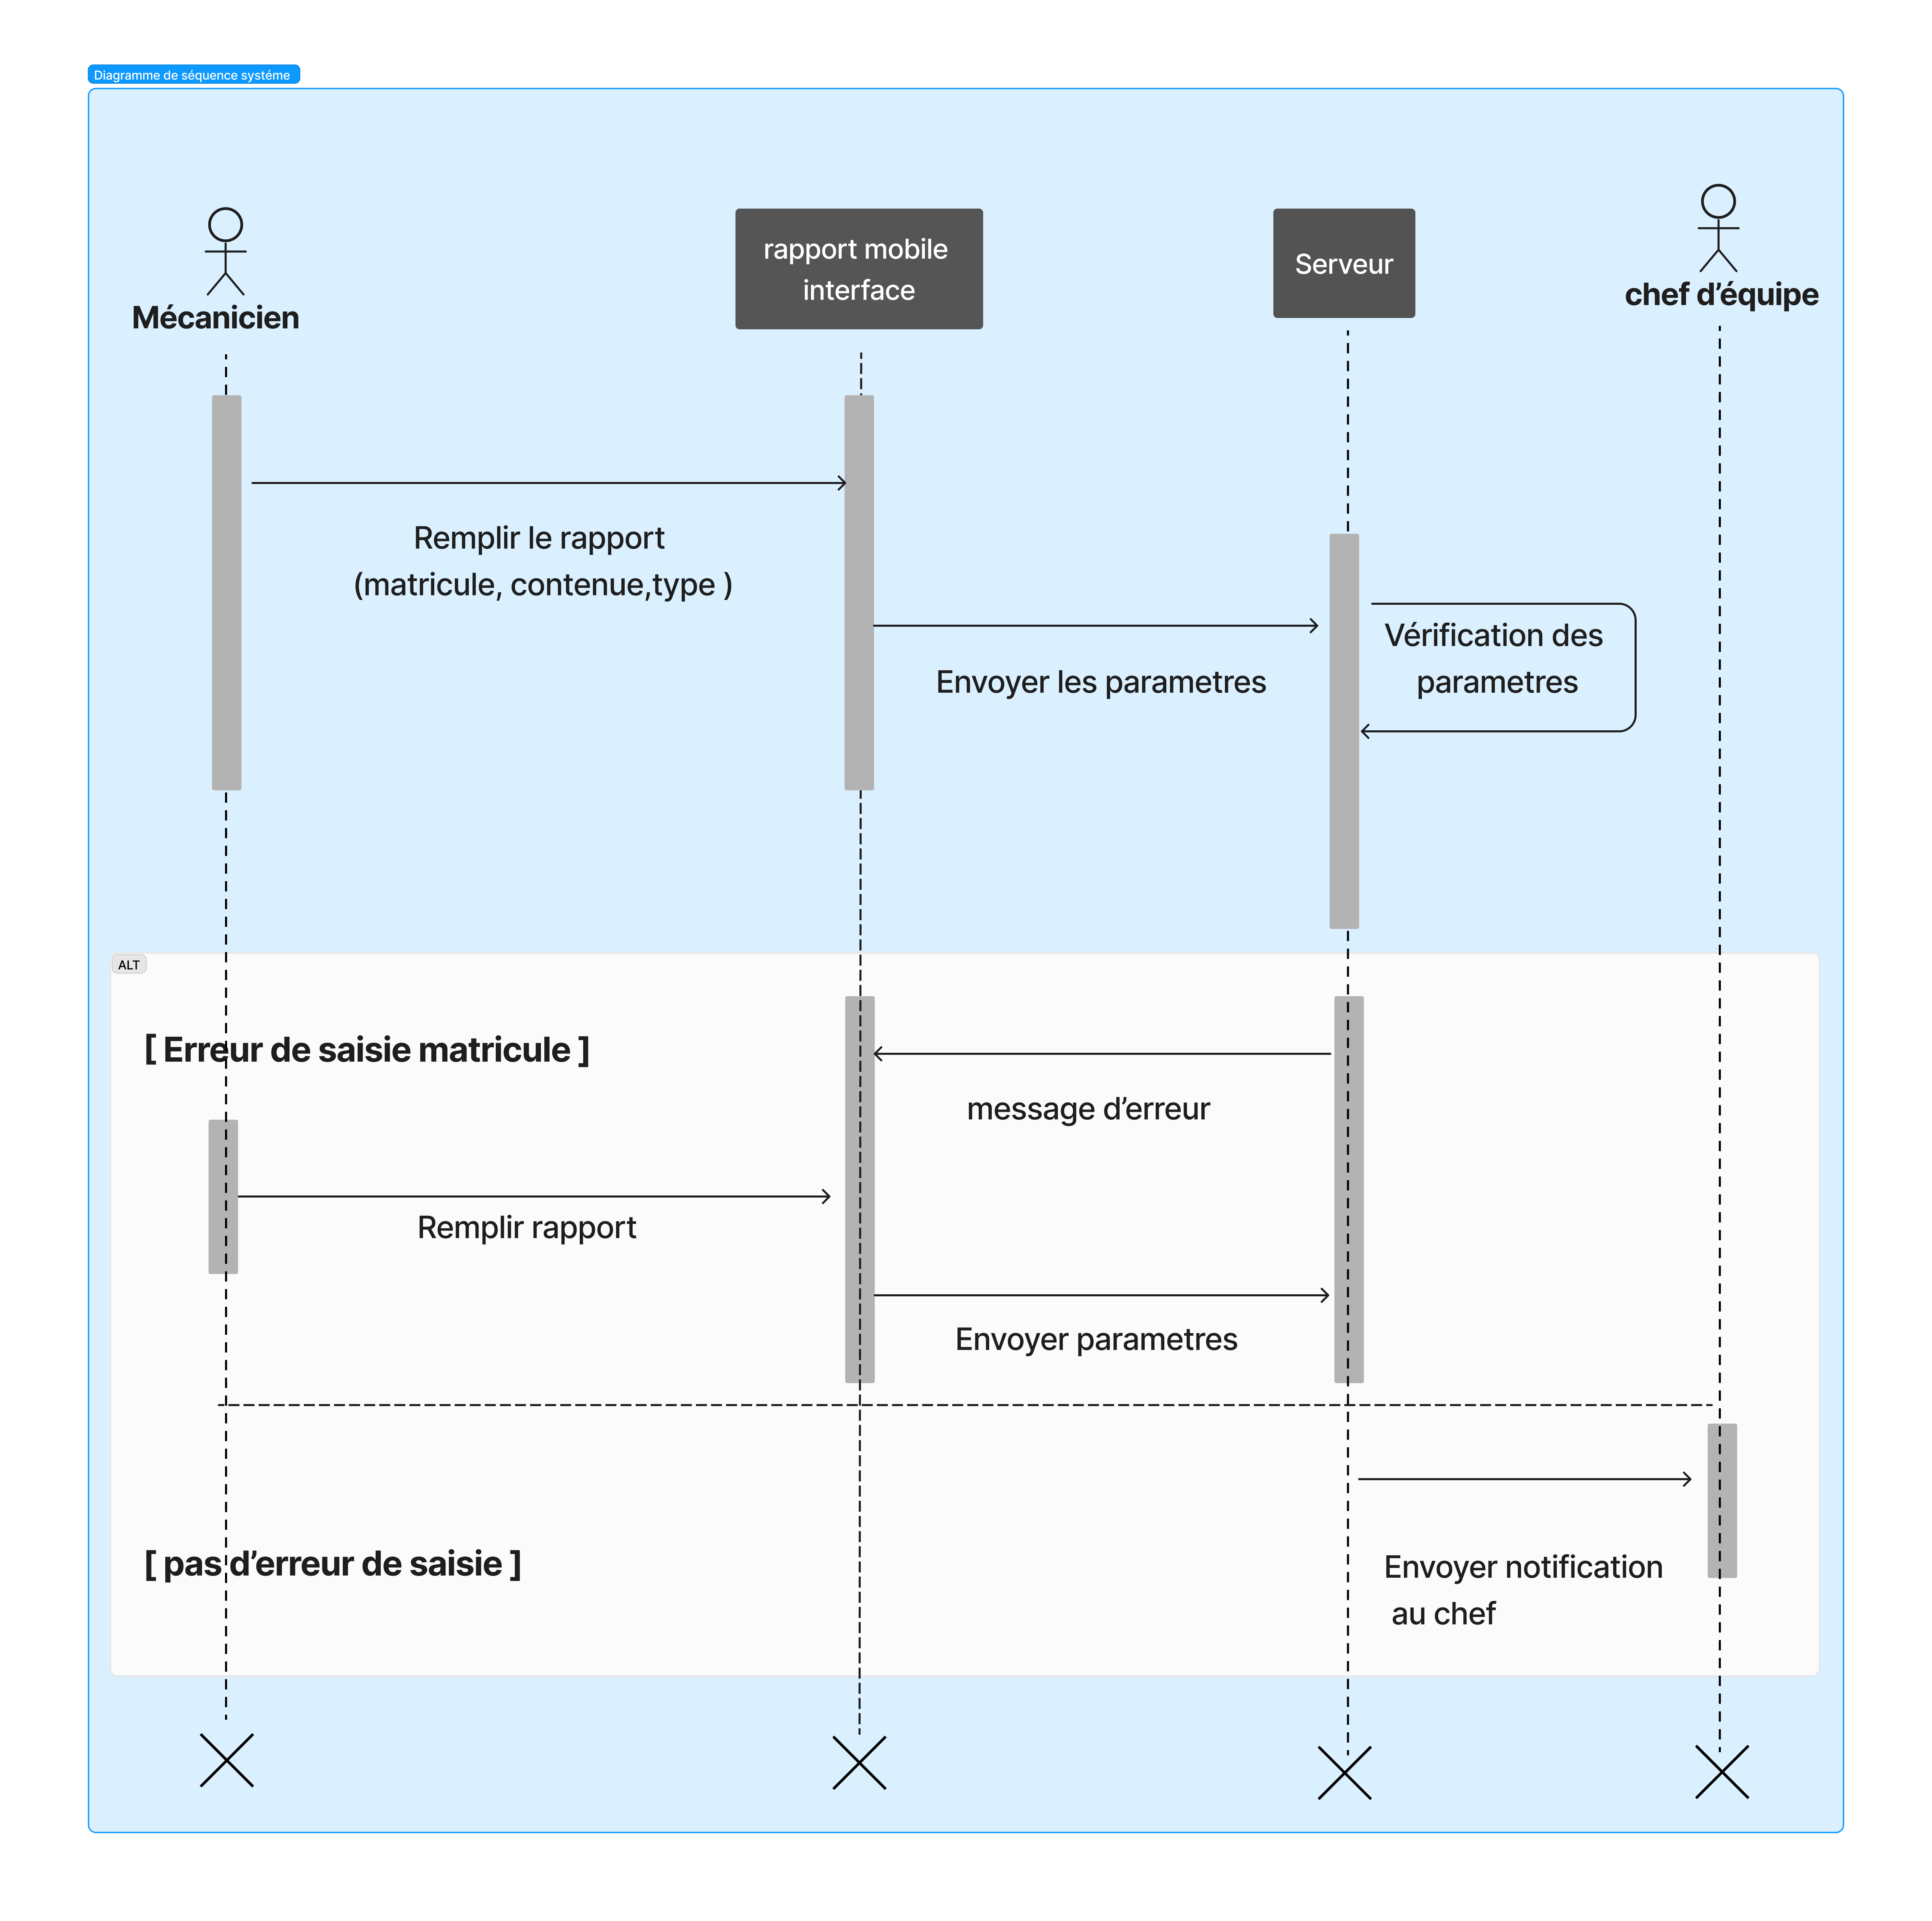
\includegraphics[width=1\textwidth,height=14cm]{chap5.images/dss rapport.png}
    \caption{Diagramme de séquence système du cas d’utilisation « Générer des rapports »}

\end{figure}


%________________________________________________________________________________________________________________
\newpage
\section{Diagramme de classes du sprint 3}

\begin{figure}[ht!]
    \centering
    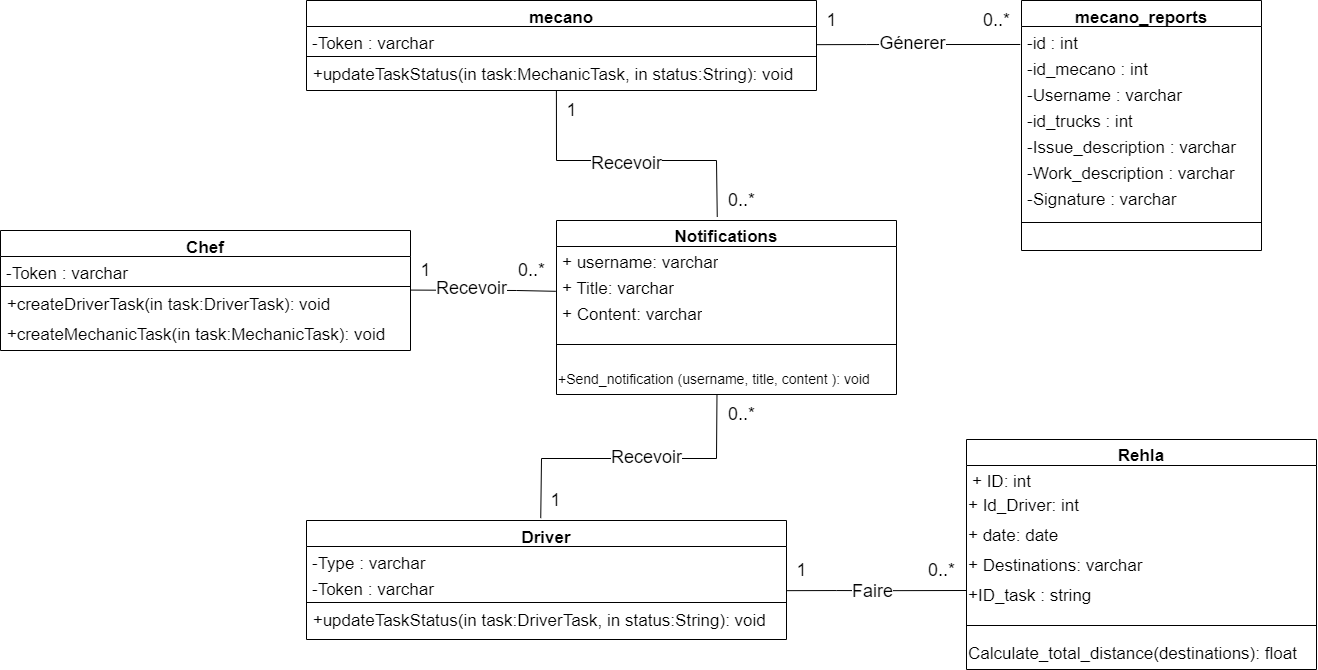
\includegraphics[width=1.1\textwidth,height=12cm]{chap5.images/class sprint 3.png}
    \caption{Diagramme de classes du sprint 3}

\end{figure}


%________________________________________________________________________________________________________________

\newpage
\section{Réalisation}

Cette section présente les interfaces développées lors du sprint 3.

\subsection{Suivi en Temps Réel par Géolocalisation}

L'interface web permet au chef d'équipe de suivre en temps réel la position des véhicules sur la carte et de surveiller les itinéraires des chauffeurs.

\begin{figure}[h!]
    \centering
    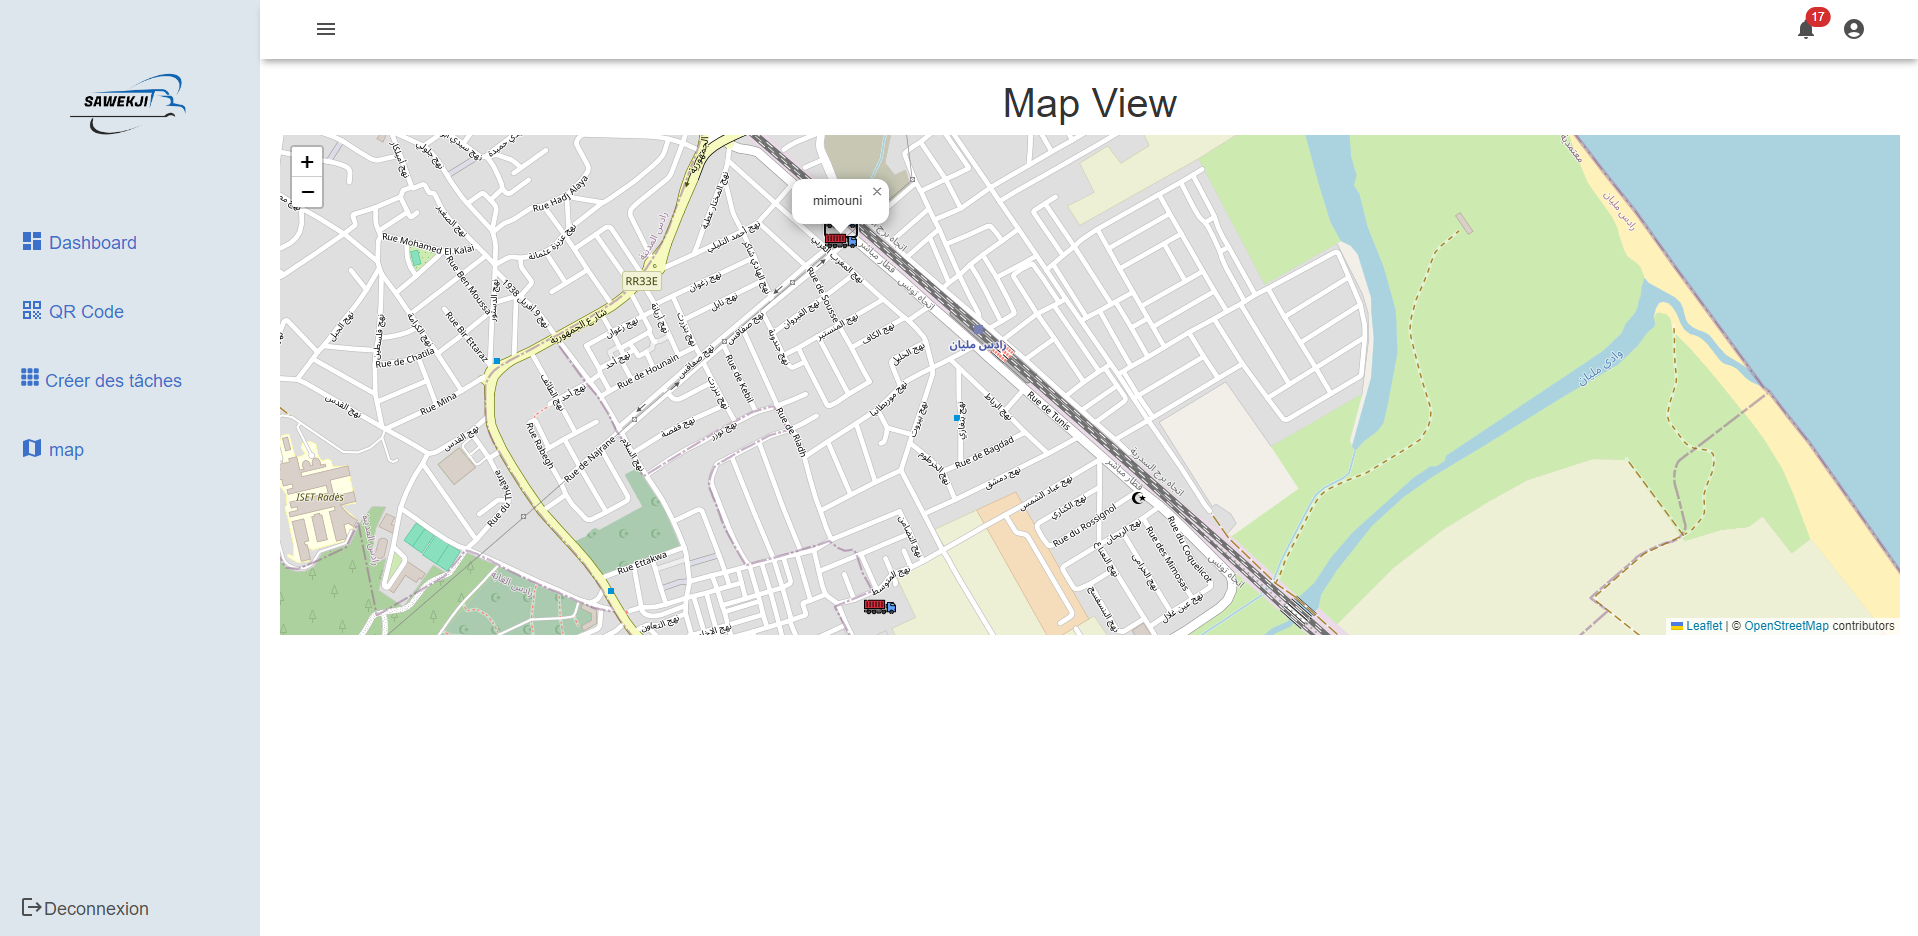
\includegraphics[width=0.9\textwidth,height=7cm]{chap5.images/map weeeb.png}
    \caption{Suivi en Temps Réel par Géolocalisation}
\end{figure}

\subsection{La planification des déplacements }

\begin{figure}[htbp]
    \centering
    \begin{minipage}{0.39\textwidth}
        \centering
        \includegraphics[width=0.8\textwidth,height=7cm]{chap5.images/trajettt.png}
        \caption{\centering{Vue du trajet}}

    \end{minipage}
    \hfill
    \begin{minipage}{0.58\textwidth}
        \raggedright
        Cette interface offre une vue d'ensemble du trajet, avec le chemin complet mis en surbrillance, la distance totale du voyage affichée en haut, et des informations sur les points de passage et la destination finale.
    \end{minipage}
\end{figure}


\newpage

\begin{figure}[htbp]
    \centering
    \begin{minipage}{0.58\textwidth}
        \raggedright
        Cette interface affiche une carte avec des stations-service (icônes de pompe à essence) pour les ravitaillements, des aires de repos pour les pauses du chauffeur, et la position actuelle du véhicule .
    \end{minipage}
    \hfill
    \begin{minipage}{0.39\textwidth}
        \centering
        \includegraphics[width=0.8\textwidth,height=7cm]{chap5.images/mazout.png}
        \caption{Carte de voyage}

    \end{minipage}
\end{figure}



\subsection{Les Notifications}

L'interface web est principalement destinée au chef d'équipe et permet de consulter les notifications relatives à l'avancement des chauffeurs et des mécaniciens. Lorsqu'un chauffeur ou un mécanicien réalise une tâche, une notification est envoyée au chef d'équipe, qui peut alors confirmer la réalisation de la tâche. Cela permet un suivi en temps réel des activités . L'interface mobile, quant à elle, est destinée aux chauffeurs, aux mécaniciens et au chef d'équipe. Elle permet de notifier ces utilisateurs à chaque fois qu'une tâche leur est assignée ou lorsqu'ils doivent accomplir une tâche spécifique. Le chef d'équipe reçoit également des notifications mobiles pour suivre l'avancement des tâches en temps réel, ce qui lui permet de rester informé même lorsqu'il n'est pas devant son ordinateur.


\begin{figure}[h!]
    \centering
    \begin{minipage}[t]{0.62\textwidth}
        \centering
        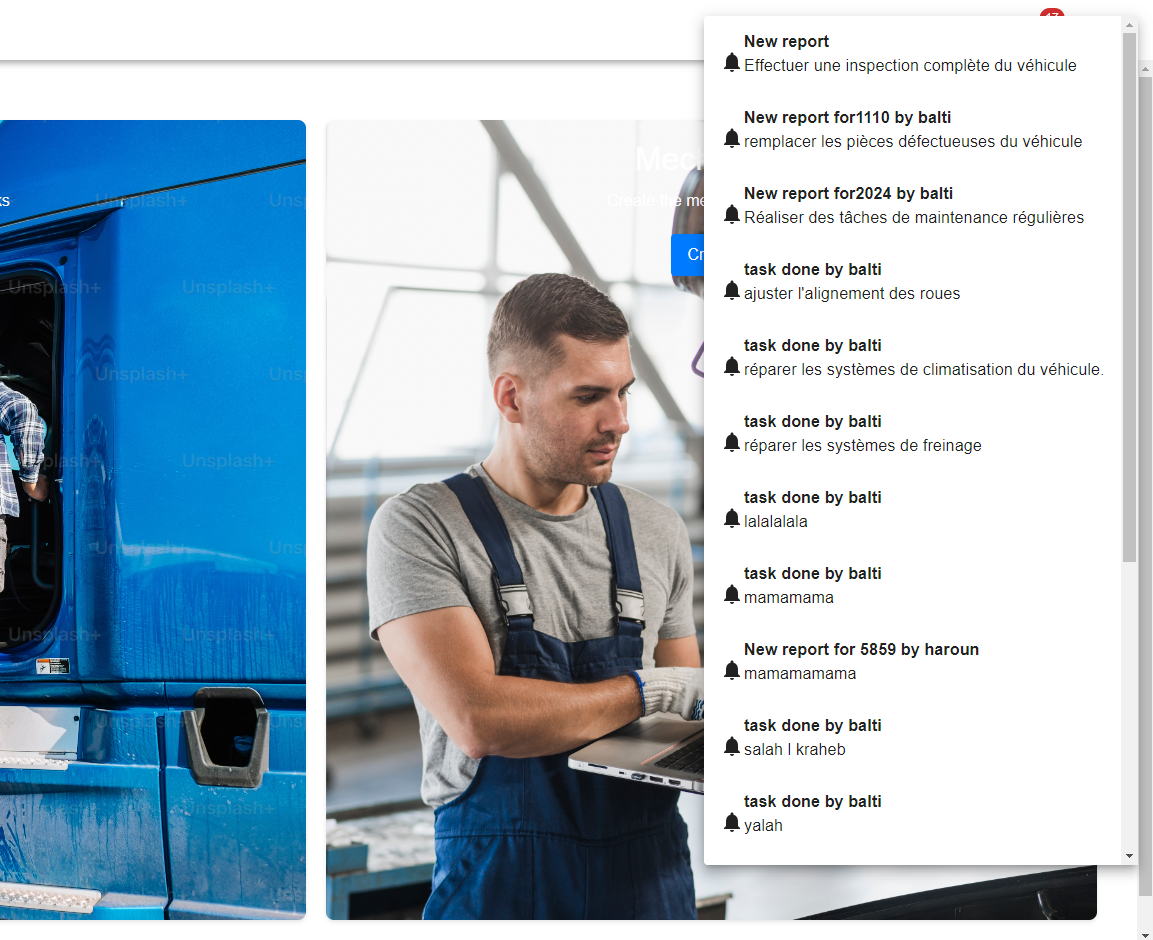
\includegraphics[width=1\textwidth, height=6cm]{chap5.images/notif web.png}
        \caption{Interface de Consultation des notifications - web »}
    \end{minipage}
    \hfill
    \begin{minipage}[t]{0.35\textwidth}
        \centering
        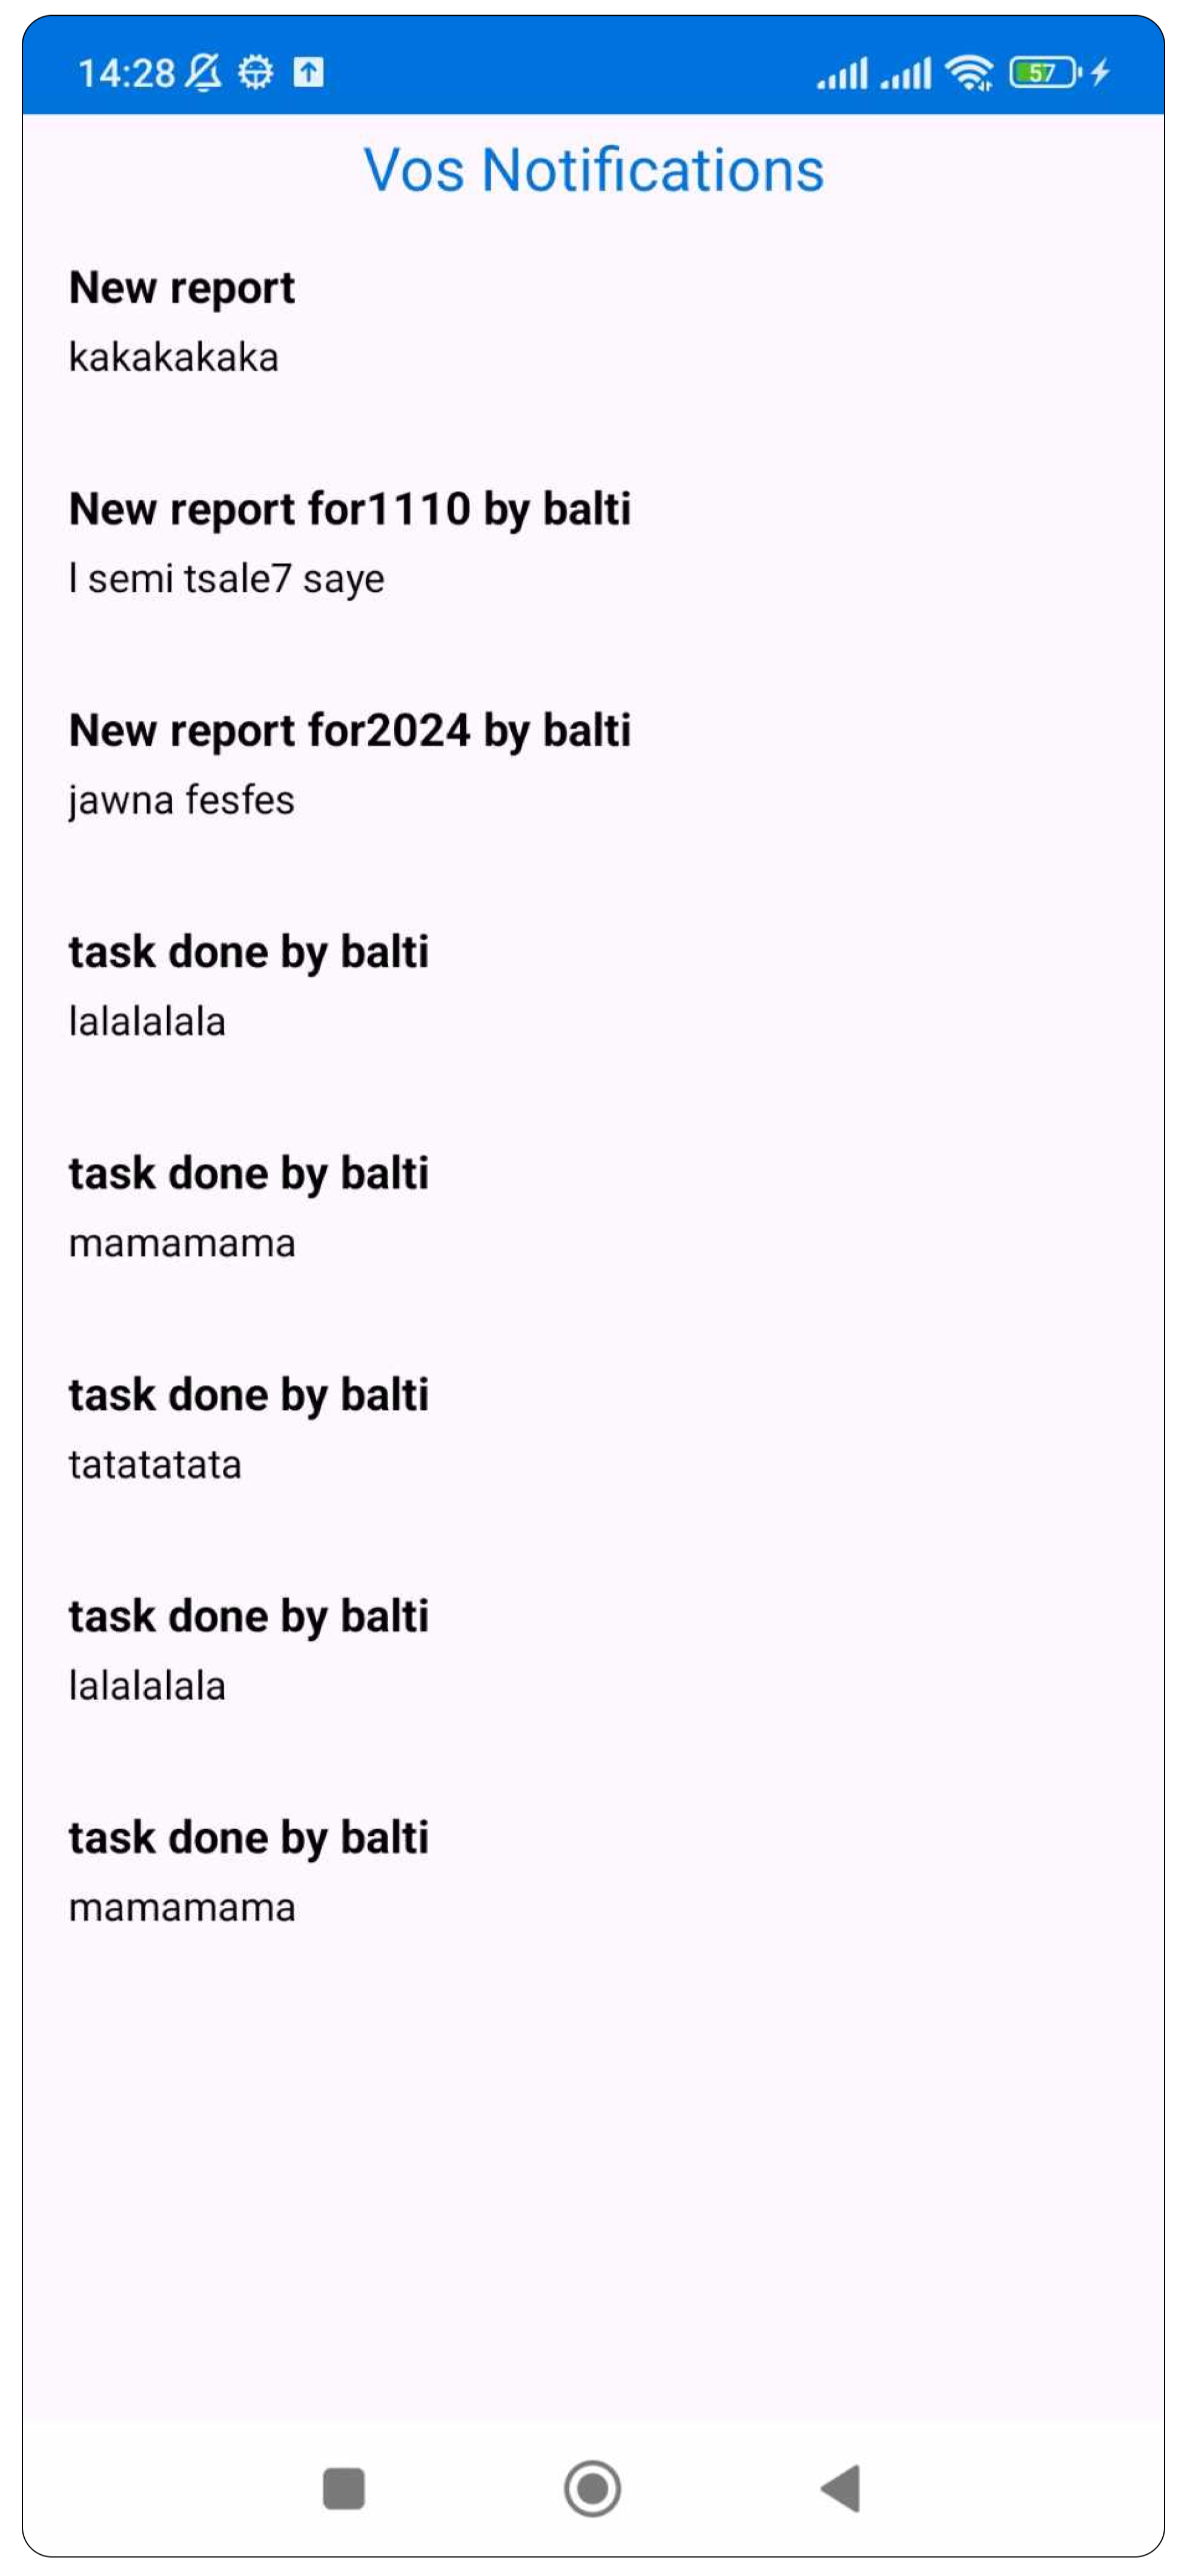
\includegraphics[width=0.8\textwidth, height=6cm]{chap5.images/notif mobile.png}
        \caption{\centering{Interface de Consultation des notifications - Mobile »}}
    \end{minipage}
\end{figure}




\newpage
\subsection{Géneration d'un Rapport}
\begin{figure}[htbp]
    \centering
    \begin{minipage}{0.58\textwidth}
        \raggedright
        Cette interface permet aux mécaniciens de saisir les informations d'un véhicule et de rédiger un rapport. Elle propose des champs pour l'ID du véhicule, la description du problème, le travail effectué et la signature du mécanicien. Des boutons permettent d'importer des photos et de sauvegarder le rapport.
    \end{minipage}
    \hfill
    \begin{minipage}{0.39\textwidth}
        \centering
        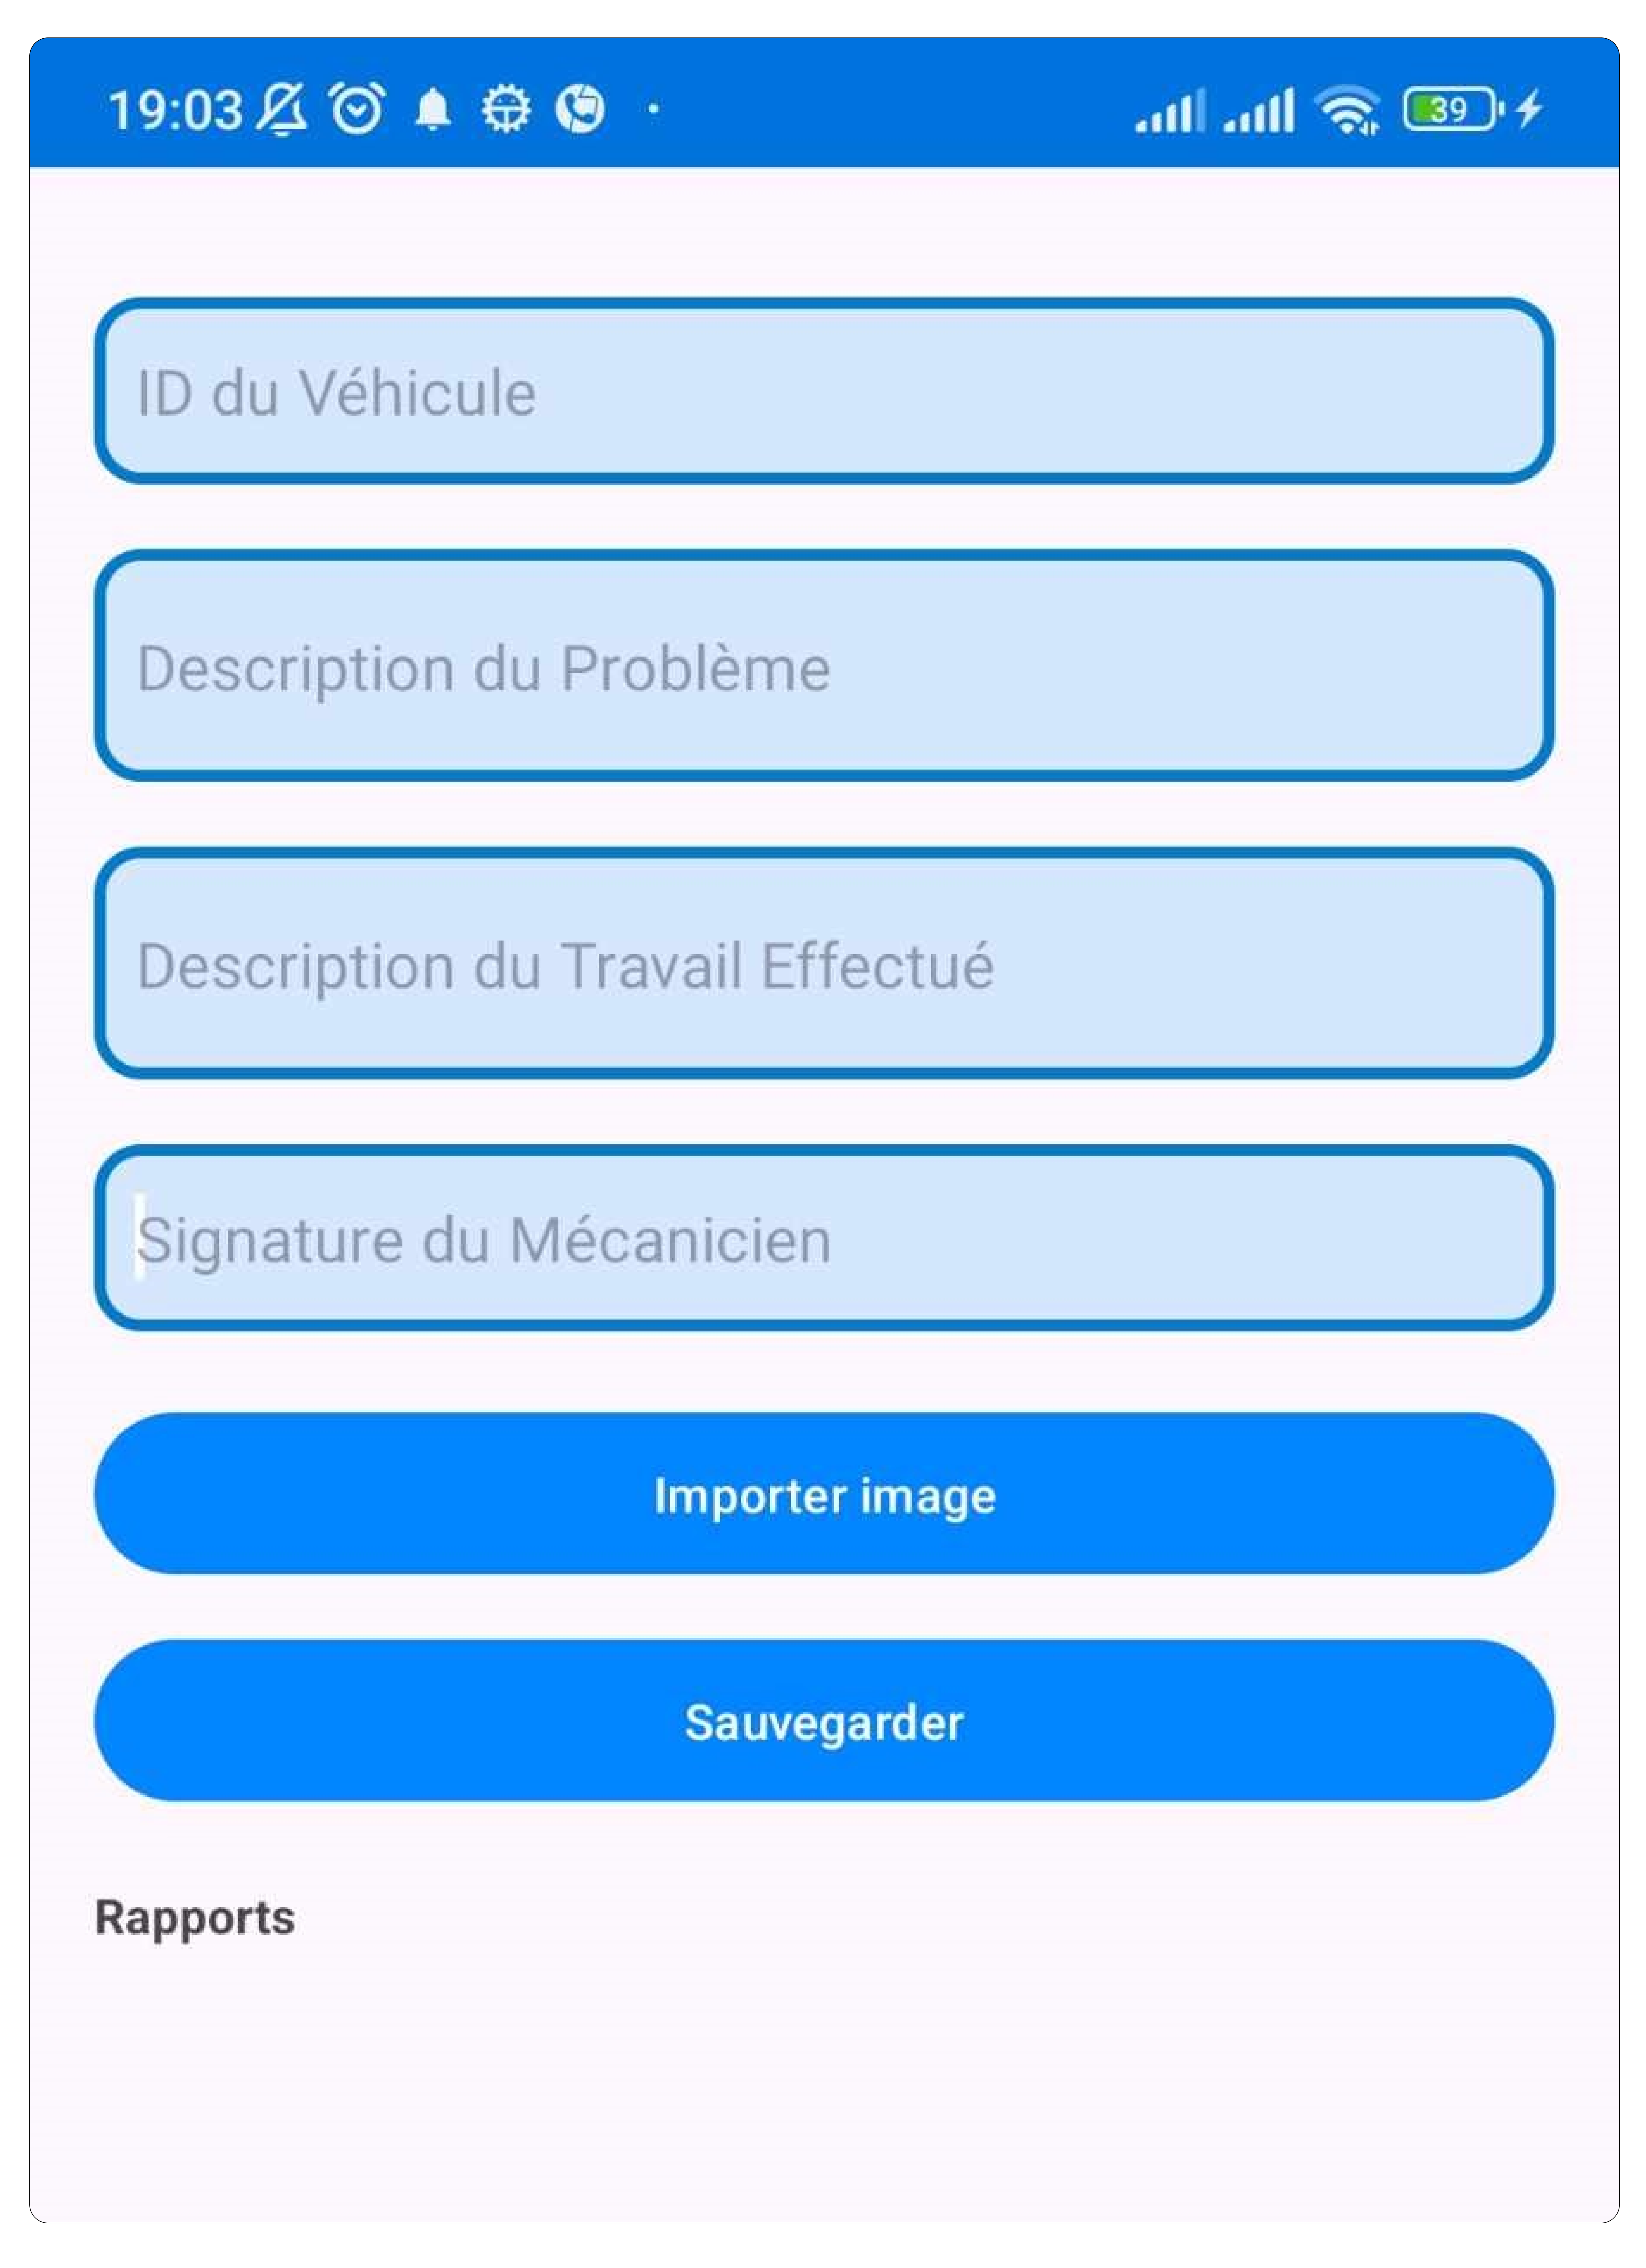
\includegraphics[width=0.7\textwidth,height=5.6cm]{chap5.images/r11.png}
        \caption{\centering Géneration de Rapport - Interface Initiale }
    \end{minipage}
\end{figure}

\begin{figure}[htbp]
    \centering
    \begin{minipage}{0.58\textwidth}
        \raggedright
        Le mécanicien a saisi le matricule et les détails du rapport d'intervention dans cette interface. Les champs de texte affichent les informations saisies.
    \end{minipage}
    \hfill
    \begin{minipage}{0.39\textwidth}
        \centering
        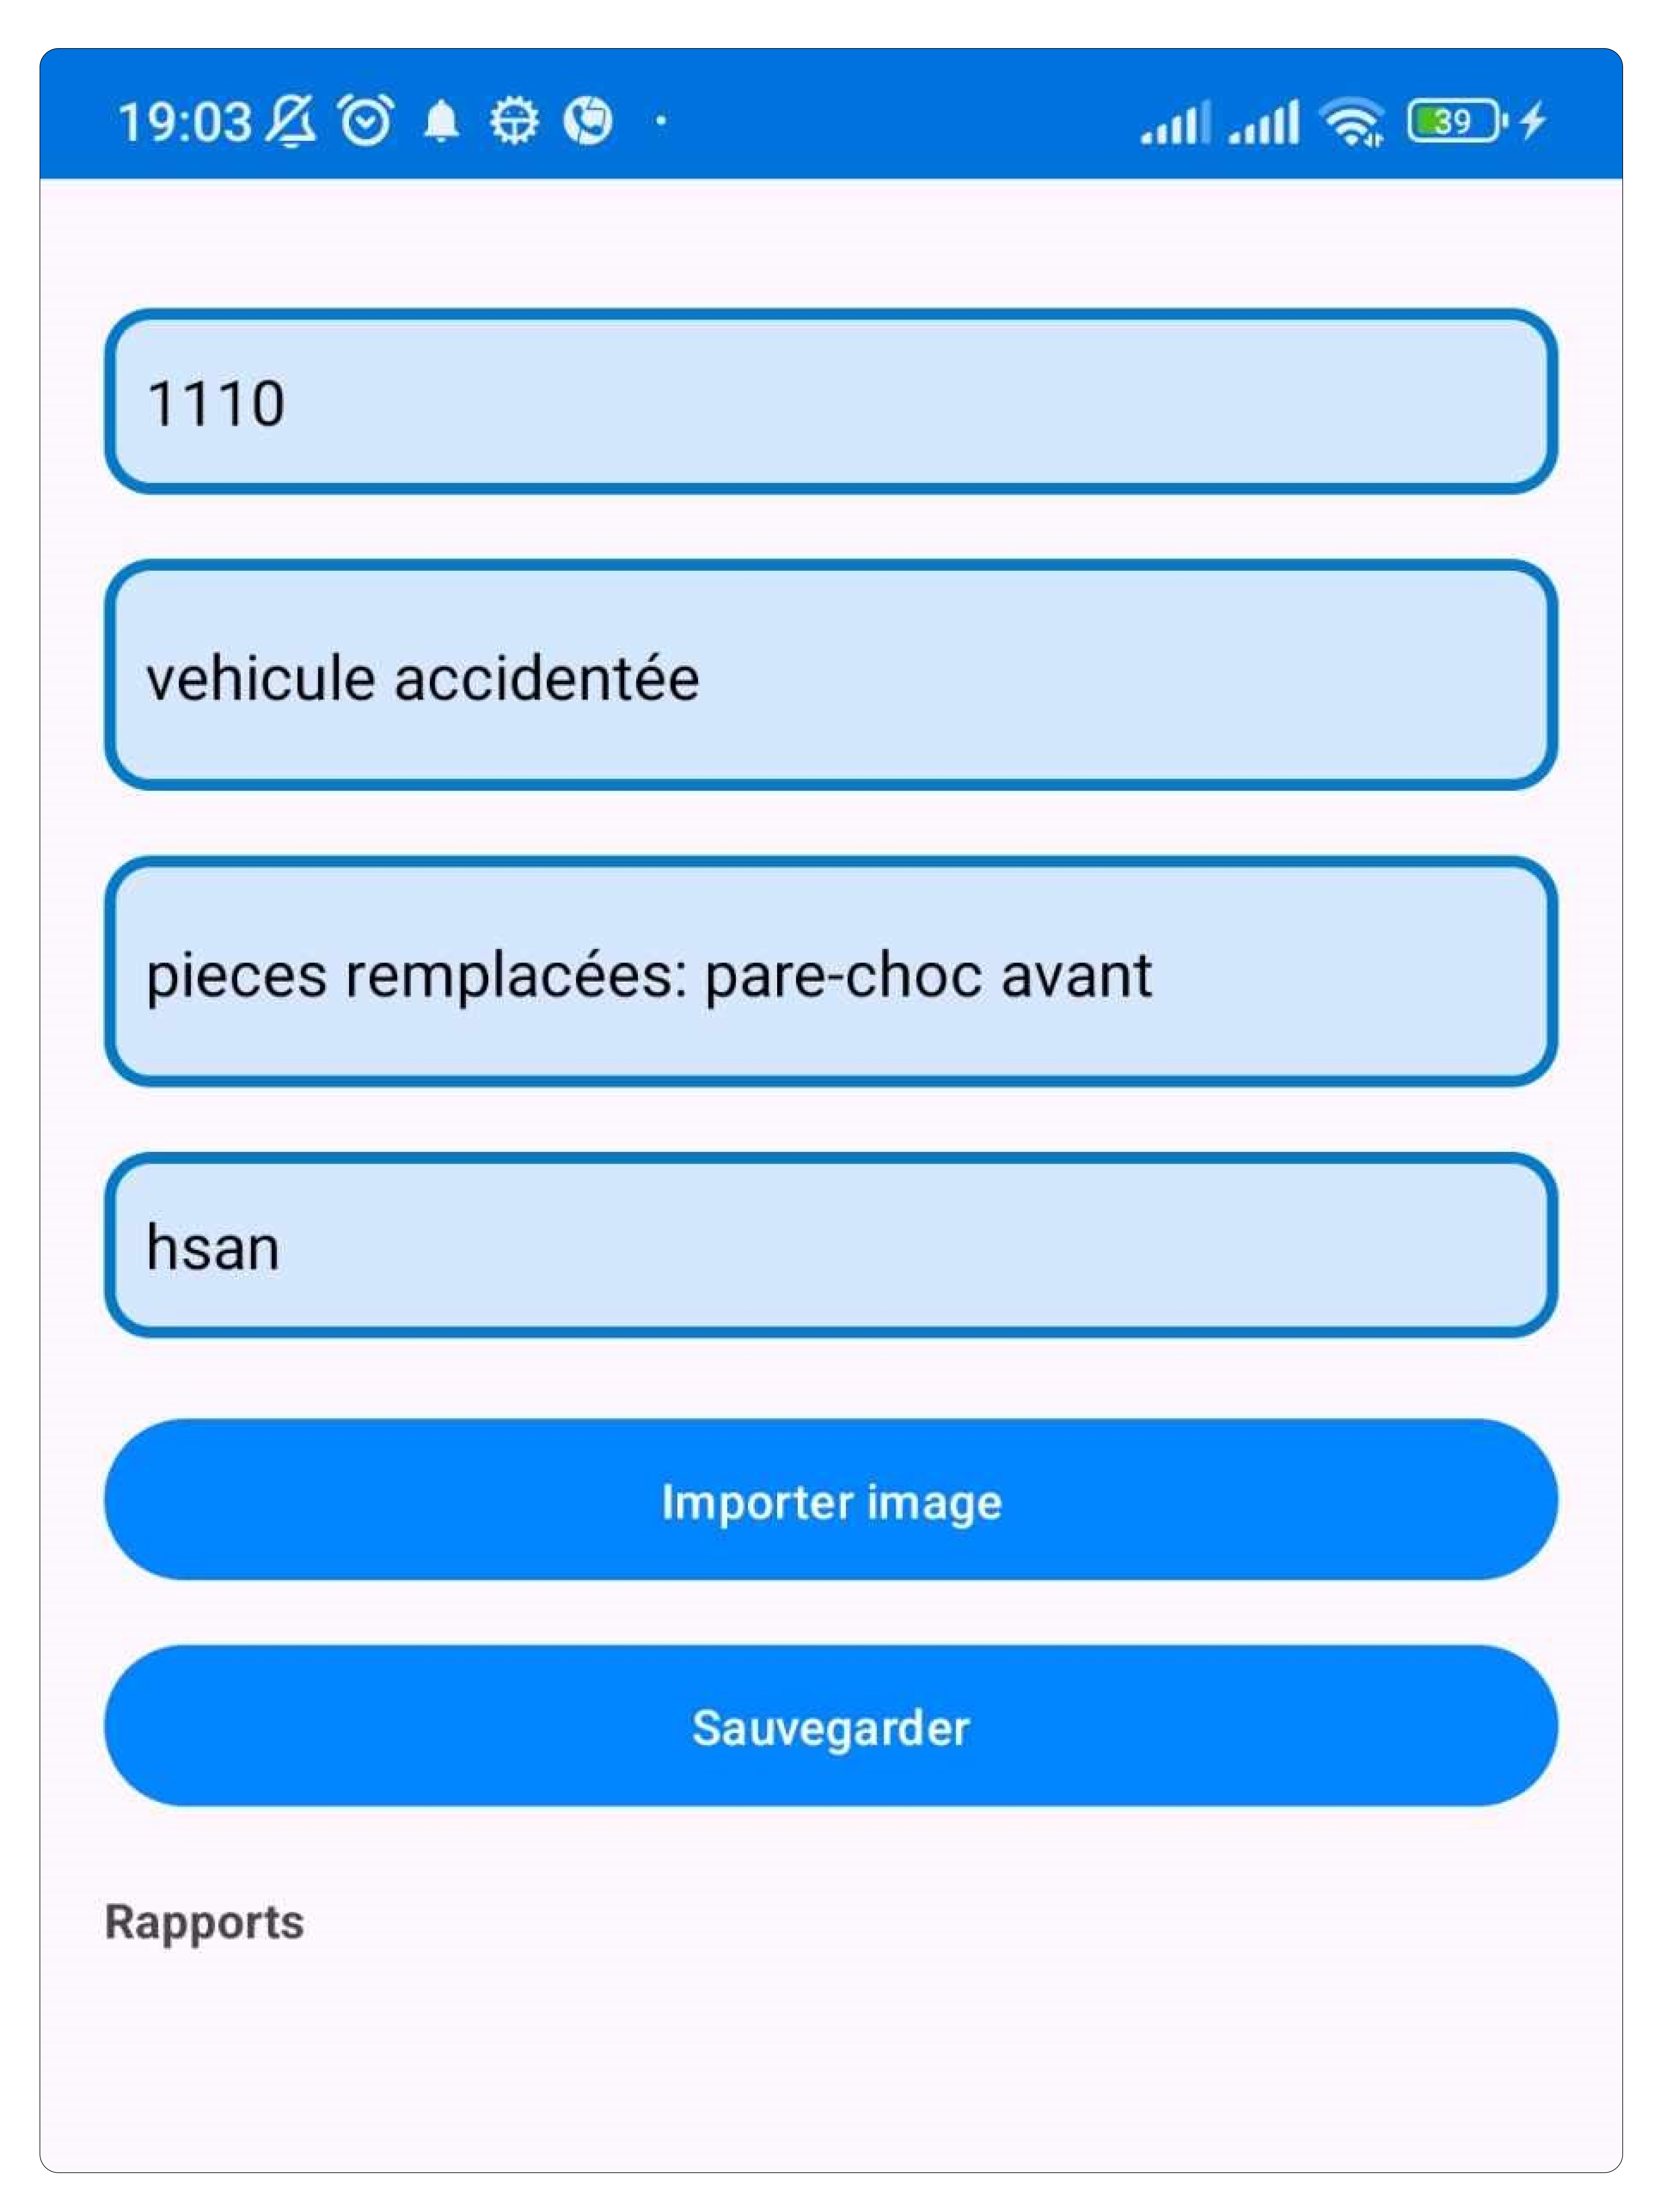
\includegraphics[width=0.7\textwidth,height=5.6cm]{chap5.images/r22.png}
        \caption{\centering Géneration de Rapport - Détails Entrés }
    \end{minipage}
\end{figure}

\begin{figure}[H]
    \centering
    \begin{minipage}{0.58\textwidth}
        \raggedright
        Cette interface affiche le rapport sauvegardé avec le matricule, les détails du problème initial et le travail effectué.
    \end{minipage}
    \hfill
    \begin{minipage}{0.39\textwidth}
        \centering
        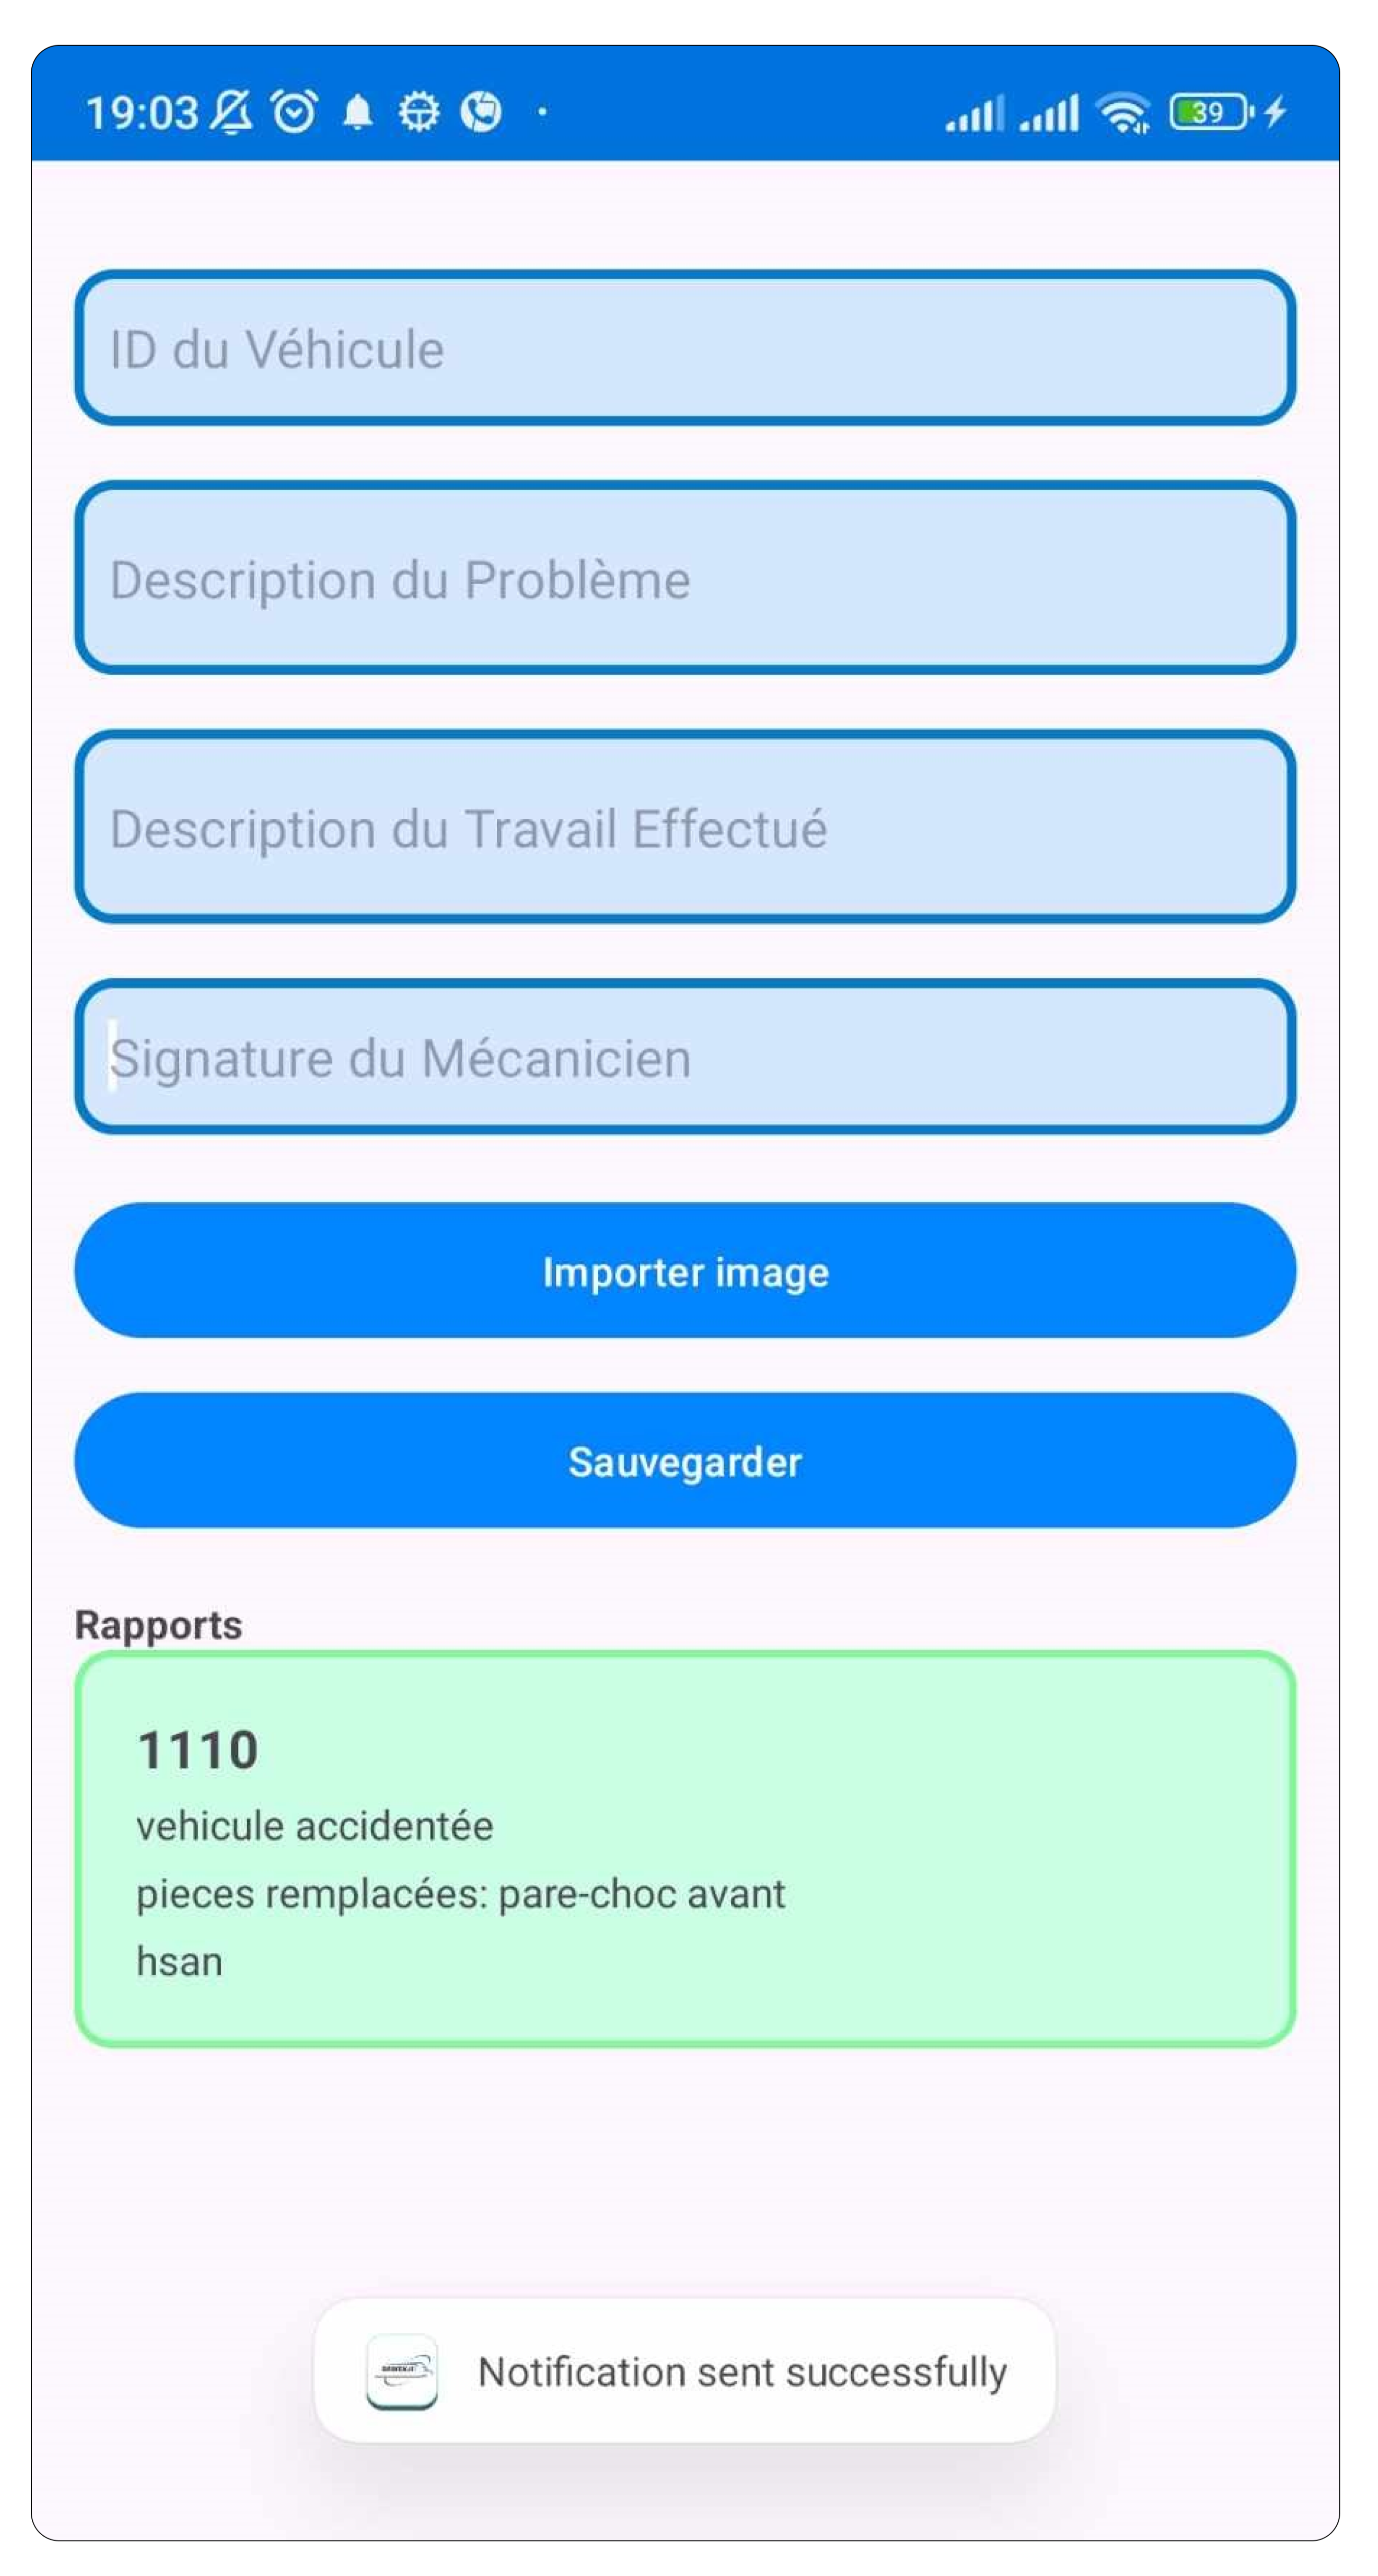
\includegraphics[width=0.7\textwidth,height=5.6cm]{chap5.images/r33.png}
        \caption{\centering Géneration de Rapport - Rapport Sauvegardé }
    \end{minipage}
\end{figure}

%________________________________________________________________________________________________________________
\newpage
\section{Rétrospective}
Pour cette rétrospective du Sprint 3, nous évaluerons les performances de notre équipe, le burndown chart et le task board nous permettront d'identifier les succès, les défis rencontrés, ainsi que les opportunités d'amélioration pour le prochain sprint.
\subsection{Burdown Chart}
Nous avons planifié un sprint de 3 semaines, avec une moyenne de 7 heures de travail par jour.

\begin{figure}[h!]
    \centering
    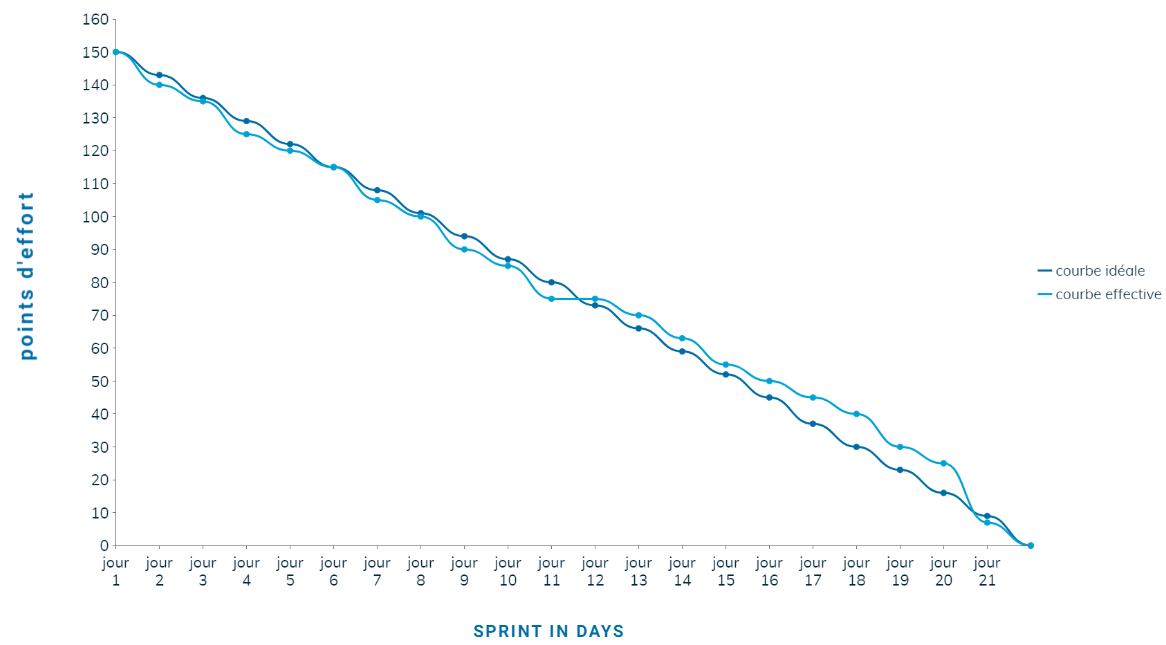
\includegraphics[width=1\textwidth, height=8.5cm]{chap5.images/Burndown chart sprint 3.png}
    \caption{ Burdown Chart du Sprint 3}

\end{figure}


\subsection{Task Bord}
La figure 4.** présente le "Task Bord" correspondant au 3ème jour du sprint 3.

\begin{figure}[h!]
    \centering
    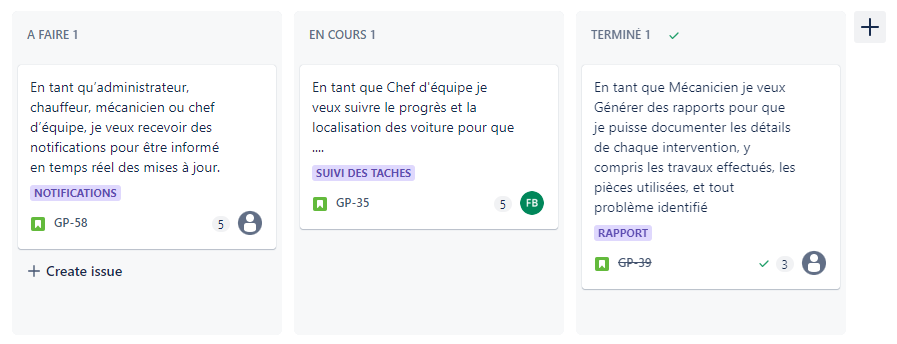
\includegraphics[width=1\textwidth,height=5.5cm]{chap5.images/task board sprint 3.png}
    \caption{ Task board du Sprint 3 }

\end{figure}
%_______________________________________________________________________________________________

\section{Tests unitaires}

\textbf{Test unitaires du cas d’utilisation « Générer des rapports » :}\\
\bigskip
Nous présentons ci-dessous le code source et le résultat de deux cas de test :\\



\textbf{1. Test de réussite :} Le test est considéré comme réussi lorsque ...\\
\textbf{2. Test d'échec :} Le test est considéré comme échoué si ...

\bigskip

\begin{figure}[h!]
    \centering
    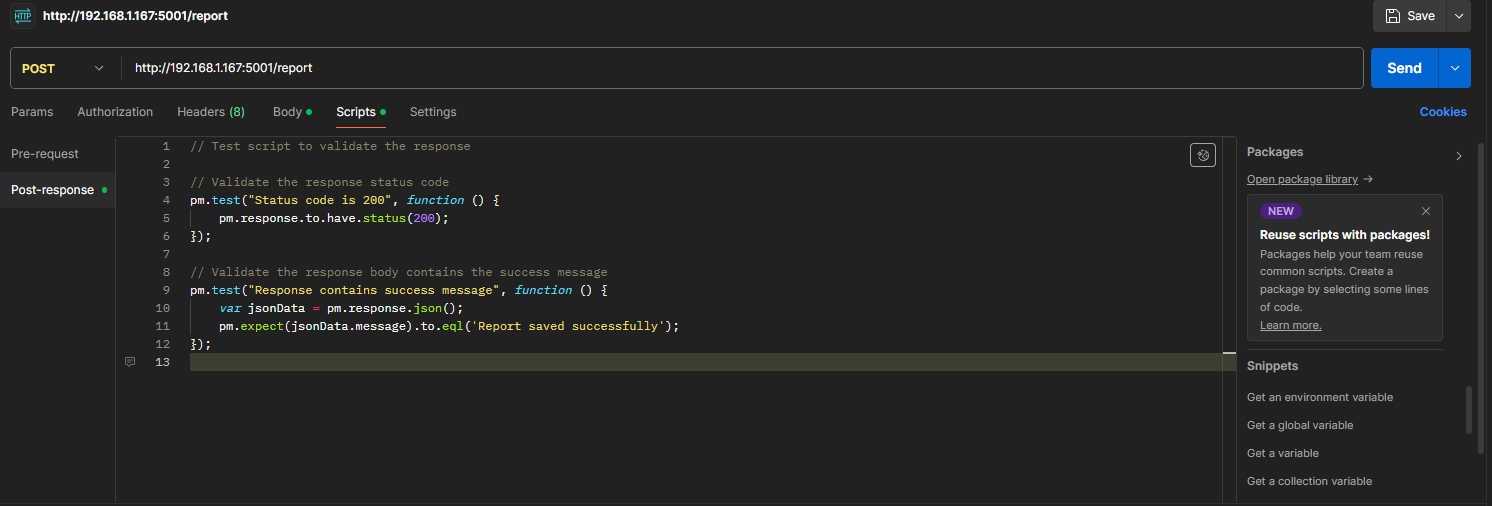
\includegraphics[width=0.8\textwidth, height=7cm]{chap5.images/source test sprint 3.png}
    \caption{ Code souce du test unitaire du cas d’utilisation « Générer des rapports » }

\end{figure}


\begin{figure}[h!]
    \centering
    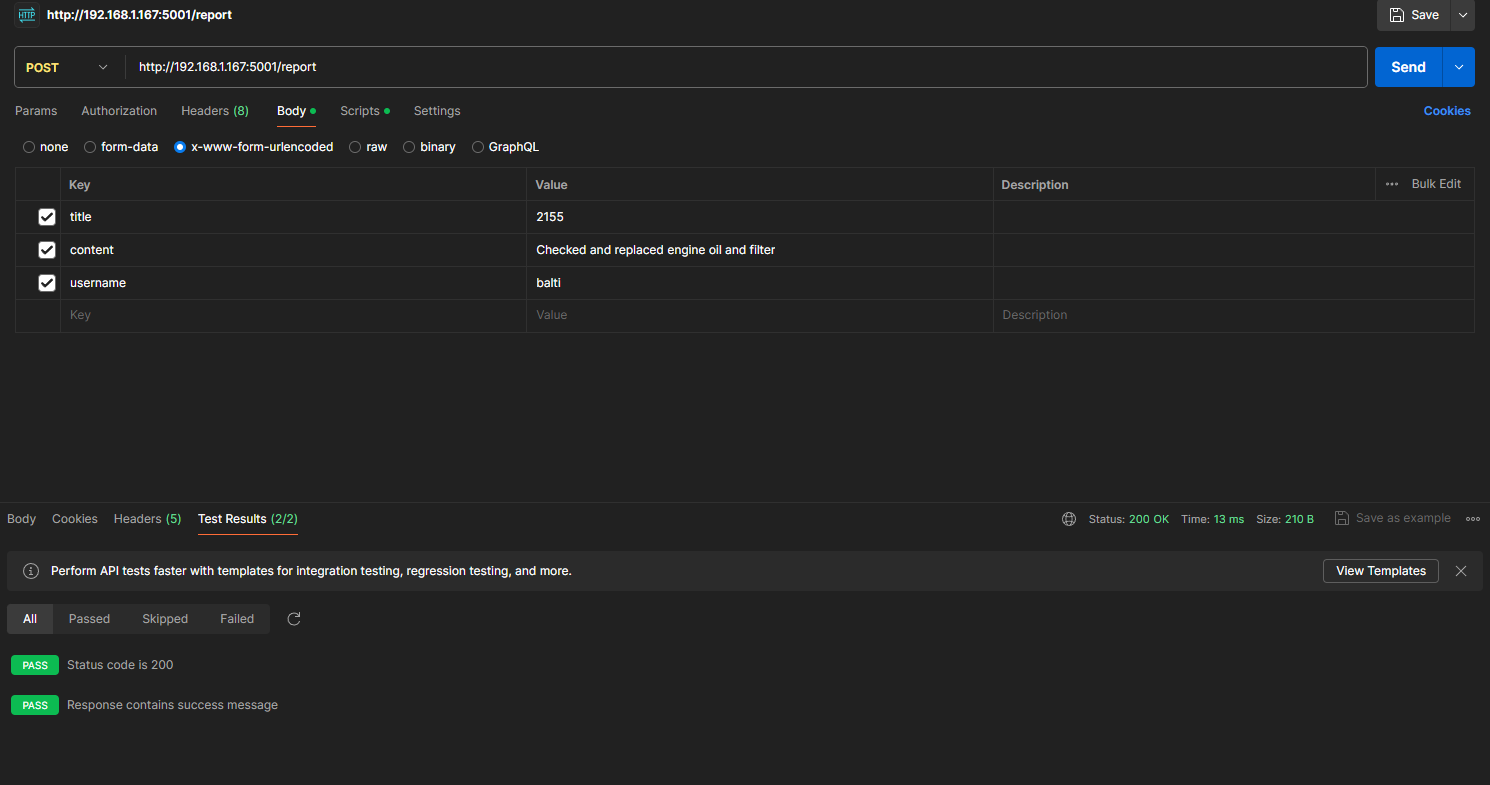
\includegraphics[width=0.8\textwidth, height=7cm]{chap5.images/succes sprint 3.png}
    \caption{ Resultat du test de réussite}

\end{figure}

\begin{figure}[h!]
    \centering
    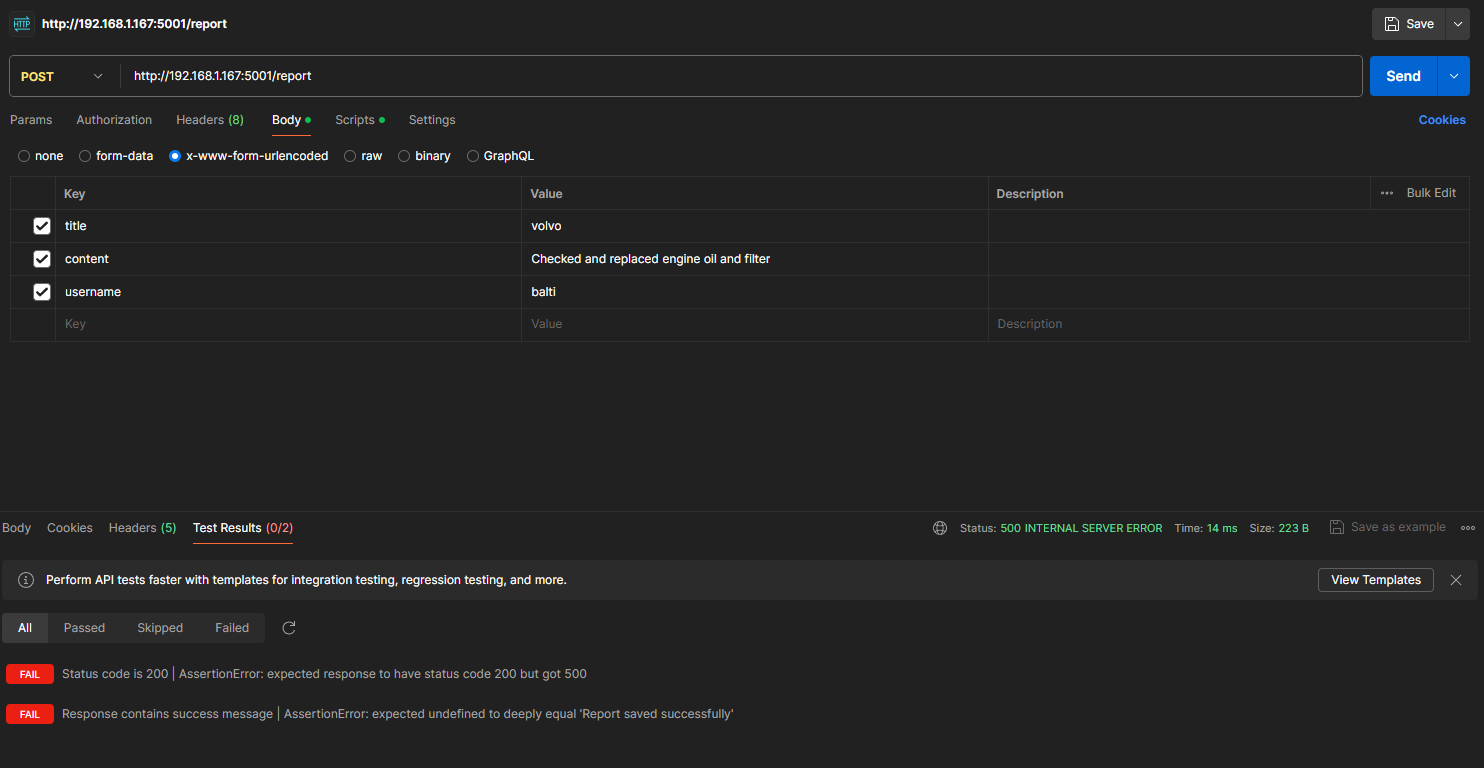
\includegraphics[width=0.8\textwidth, height=7cm]{chap5.images/fail sprint 3.png}
    \caption{ Resultat du test d'échec }

\end{figure}
%_______________________________________________________________________________________________
\newpage
\section*{Conclusion}
\addcontentsline{toc}{section}{Conclusion}
\bigskip
\begin{sloppypar}
    Ce sprint a consolidé le suivi en temps réel, la planification des déplacements, les notifications et la génération de rapports. Les interfaces web et mobile ont renforcé la coordination, permettant au chef d'équipe de suivre les véhicules et aux chauffeurs de gérer efficacement les itinéraires. La simplification de la génération de rapports a amélioré l'efficacité des mécaniciens. Les ajustements basés sur les outils de suivi préparent efficacement la transition vers le dernier sprint.
\end{sloppypar}



